%%%%%%%%%%%%%%%%%%%%%%%%%%%%%%%%%%%%%%%%%%%%%%%%%%%%%%%%%%%%%%%%%%%%%%%%%%%%%
%% Documento base para escrita de monografias e relatórios do LabEPI.      %%
%% Aluno: Nome do Aluno <aluno@email.com>                                  %%
%% Orientador: Nome do Orientador <orientador@email.com>                   %%
%%%%%%%%%%%%%%%%%%%%%%%%%%%%%%%%%%%%%%%%%%%%%%%%%%%%%%%%%%%%%%%%%%%%%%%%%%%%%

%%%%%%%%%%%%%%%%%%%%%%%%%%%%%%%%%%%%%%%%%%%%%%%%%%%%%%%%%%%%%%%%%%%%%%%%%%%%%
%% DECLARAÇÂO DAS OPÇÔES E DO TIPO DO DOCUMENTO                            %%
%%%%%%%%%%%%%%%%%%%%%%%%%%%%%%%%%%%%%%%%%%%%%%%%%%%%%%%%%%%%%%%%%%%%%%%%%%%%%
% Definição dos possíveis tipos de documento
\def\doctypem{m}
\def\doctyper{r}

% Escolha do tipo de documento
%\def\doctype{m} % Para monografias
\def\doctype{r} % Para relatórios técnicos

\if\doctype\doctypem           % Se é do tipo monografia
\documentclass[twoside,a4paper,11pt]{book}
\fi
\if\doctype\doctyper           % Se é do tipo relatório
\documentclass[a4paper,11pt]{report}
\fi

%%%%%%%%%%%%%%%%%%%%%%%%%%%%%%%%%%%%%%%%%%%%%%%%%%%%%%%%%%%%%%%%%%%%%%%%%%%%%
%% PACOTES UTILIZADOS                                                      %%
%%%%%%%%%%%%%%%%%%%%%%%%%%%%%%%%%%%%%%%%%%%%%%%%%%%%%%%%%%%%%%%%%%%%%%%%%%%%%
%\usepackage[usenames,dvips]{color}
%\usepackage{ae}
%\usepackage{afterpage}
%\usepackage{appendix}
%\usepackage{eukdate}
%\usepackage{listings}
%\usepackage{lscape}
%\usepackage{multirow}
%\usepackage{nomencl}
%\usepackage{pslatex}
%\usepackage{rotating}
%\usepackage{setspace}
%\usepackage{supertabular}
%\usepackage{tabularx}
%\usepackage{tikz}
%\usepackage{url}
%\usepackage{verbatim}
%\usepackage{showframe}
\usepackage[top=3.5cm,bottom=3.5cm,left=3cm,right=3cm]{geometry}
%\usepackage[square]{natbib}
\usepackage{natbib}
\usepackage[labelfont=bf,font=small]{caption}
\usepackage[plain,chapter]{algorithm}
\usepackage[portuges,brazil]{babel}
\usepackage[utf8]{inputenc}
\usepackage{algorithmic}
\usepackage{amsmath}
\usepackage{amssymb}
\usepackage{amsthm}
\usepackage{booktabs}
\usepackage{enumitem}
\usepackage{fancyhdr}
\usepackage{graphicx}
\usepackage{indentfirst}
\usepackage{lineno}
\usepackage{longtable}
\usepackage{paralist}
\usepackage{thmtools}
\usepackage{lastpage}
\usepackage{imakeidx}
\usepackage[pagebackref,breaklinks]{hyperref}
\usepackage{titlesec}
\usepackage{pgfgantt}

%%%%%%%%%%%%%%%%%%%%%%%%%%%%%%%%%%%%%%%%%%%%%%%%%%%%%%%%%%%%%%%%%%%%%%%%%%%%%
%% PARÂMETROS                                                              %%
%%%%%%%%%%%%%%%%%%%%%%%%%%%%%%%%%%%%%%%%%%%%%%%%%%%%%%%%%%%%%%%%%%%%%%%%%%%%%

%%%%%%%%%%%%%%%%%%%%%%%%%%%%%%%%%%%%%%%%%%%%%%%%%%%%%%%%%%%%%%%%%%%%%%%%%%%%%
%% INÍCIO DO ARQUIVO DE COMANDOS                                           %%
%%%%%%%%%%%%%%%%%%%%%%%%%%%%%%%%%%%%%%%%%%%%%%%%%%%%%%%%%%%%%%%%%%%%%%%%%%%%%

% Muda o estilo do cabeçalho dos capítulos so for um relatório
\if\doctype\doctyper           % Se é do tipo relatório
\titleformat{\chapter}{\normalfont\huge\bf}{\thechapter.}{20pt}{\huge\bf}
\fi

\newcommand{\limparpagina}{%
\if\doctype\doctypem           % Se é do tipo monografia
  \cleardoublepage
\fi
\if\doctype\doctyper           % Se é do tipo relatório
  \clearpage
\fi}

% Infenização
\hyphenation{net-works lay-out}

% Comandos próprios
\newcommand*\pct{\scalebox{.9}{\%}}

% Configuração do ambiente Verbatim do fancyvrb
\fvset{fontsize=\small,frame=single,xleftmargin=1mm,xrightmargin=1mm}

% Configuração de diagramas de Gantt
\ganttset{%
  canvas/.append style={fill=none, dotted},
  %vgrid={draw={none}, dotted},
  vgrid,
  hgrid,
  today label=Prazo,
  group height=.3,
  group left shift=0,
  group right shift=0,
  group peaks={0}{}{},
  group/.style={draw=black,fill=black},    
  bar height=.3,
  bar/.style={fill=black},
  progress label text={#1\pct},
  title height=1}

\newcommand{\citacao}[2]{%
\begin{flushright}
\footnotesize
\parbox{0.95\textwidth}{\flushright{\it``#1''\\ \scriptsize #2}}
\end{flushright}}

\DeclareMathOperator*{\argmin}{arg\,min}
\DeclareMathOperator*{\argmax}{arg\,max}

\newcommand{\definirtitulo}[1]{\newcommand{\titulo}{#1}}
\newcommand{\definirtitulocurto}[1]{\newcommand{\titulocurto}{#1}}

% Algoritmos
\floatname{algorithm}{Algoritmo}
\renewcommand{\listalgorithmname}{Lista de Algoritmos}

\renewcommand{\algorithmicindent}{2.0em}
\renewcommand{\algorithmicrequire}{\textbf{algoritmo}}
\renewcommand{\algorithmicensure}{\textbf{fim algoritmo}}
\renewcommand{\algorithmicreturn}{\textbf{retorne}}
\renewcommand{\algorithmicor}{\textbf{ou}}
\renewcommand{\algorithmicand}{\textbf{e}}
\renewcommand{\algorithmicend}{\textbf{fim}}
\renewcommand{\algorithmicif}{\textbf{se}}
\renewcommand{\algorithmicthen}{\textbf{ent\~ao}}
\renewcommand{\algorithmicfor}{\textbf{para}}
\renewcommand{\algorithmicforall}{\textbf{para cada}}
\renewcommand{\algorithmicrepeat}{\textbf{repita}}
\renewcommand{\algorithmicuntil}{\textbf{enquanto}}
\renewcommand{\algorithmicwhile}{\textbf{enquanto}}
\renewcommand{\algorithmicdo}{\textbf{fa\c{c}a}}

% Cabeçalho e rodapé
\renewcommand{\thefootnote}{[\roman{footnote}]}
\setlength{\headheight}{14.5pt}

\fancypagestyle{labepi}{%
\fancyhead{}
\fancyfoot{}
\if\doctype\doctypem           % Se é do tipo monografia
  \fancyhead[LO]{\bf\nouppercase \rightmark}
  \fancyhead[RO]{\bf\thepage}
  \fancyhead[LE]{\bf\thepage}
  \fancyhead[RE]{\bf\nouppercase \leftmark}
\fi
\if\doctype\doctyper           % Se é do tipo relatório
  \fancyhead[R]{\bf\thepage}
  \fancyhead[L]{\bf\titulocurto}
\fi
\renewcommand{\headrulewidth}{0pt}
\renewcommand{\footrulewidth}{0pt}}

\fancypagestyle{plain}{%
\fancyhead{}
\fancyfoot{}
\fancyhead[R]{\bf\thepage}
\fancyhead[L]{\bf\titulocurto}
\renewcommand{\headrulewidth}{0pt}
\renewcommand{\footrulewidth}{0pt}}

% Teoremas
\declaretheoremstyle[
  spaceabove=6pt,
  spacebelow=6pt,
  headfont=\normalfont\bfseries,
  notefont=\mdseries,
  notebraces={(}{)},
  bodyfont=\normalfont,
  postheadspace=1em,
  qed=$\square$,
  numberwithin=chapter
]{thmsty}

\declaretheorem[style=thmsty,name=Algoritmo]{algoritmo}

\declaretheorem[style=thmsty,name=Definição]{definicao}
\declaretheorem[style=thmsty,name=Premissa]{premissa}

\declaretheorem[style=thmsty,name=Afirmação]{afirmacao}
\declaretheorem[style=thmsty,name=Observação]{observacao}
\declaretheorem[style=thmsty,name=Corolário]{corolario}
\declaretheorem[style=thmsty,name=Lema]{lema}
\declaretheorem[style=thmsty,name=Teorema]{teorema}

\declaretheorem[style=thmsty,name=Nota]{nota}

\renewcommand{\qedsymbol}{{\bf C.Q.D.}}

% Bibliografia
\newcommand{\backrefnotcited}{\relax} %(Not cited.)
\newcommand{\backrefcitedsingle}[1]{\\(Citado na página~#1)}
\newcommand{\backrefcitedmultiple}[1]{\\(Citado nas páginas~#1)}
\renewcommand{\backreftwosep}{ e~}
\renewcommand{\backreflastsep}{ e~}
\renewcommand*{\backref}[1]{}
\renewcommand*{\backrefalt}[4]{%
\ifcase #1
  \backrefnotcited
\or
  \backrefcitedsingle{#2}
\else
  \backrefcitedmultiple{#2}
\fi}

% Índice
\makeindex[intoc,options={-s labepi.ist}]

\hypersetup{colorlinks,linkcolor=blue,citecolor=blue}

\index{recorrencia@recorrência|see{recursividade}}
\index{recursividade|see{recorrência}}

%%%%%%%%%%%%%%%%%%%%%%%%%%%%%%%%%%%%%%%%%%%%%%%%%%%%%%%%%%%%%%%%%%%%%%%%%%%%%
%% FIM DO ARQUIVO DE COMANDOS                                              %%
%%%%%%%%%%%%%%%%%%%%%%%%%%%%%%%%%%%%%%%%%%%%%%%%%%%%%%%%%%%%%%%%%%%%%%%%%%%%%
       % Comandos próprios

%%%%%%%%%%%%%%%%%%%%%%%%%%%%%%%%%%%%%%%%%%%%%%%%%%%%%%%%%%%%%%%%%%%%%%%%%%%%%
%% INÍCIO DO DOCUMENTO                                                     %%
%%%%%%%%%%%%%%%%%%%%%%%%%%%%%%%%%%%%%%%%%%%%%%%%%%%%%%%%%%%%%%%%%%%%%%%%%%%%%

\definirtitulo{%
Modelo de Referência para Escrita de Monografias e Relatórios do LabEPI}

\definirtitulocurto{Modelo de Monografias e Relatórios do LabEPI}

\begin{document}

% Numeração de linhas para auxiliar nas correções (comentar na versão final)
\linenumbers

\pagestyle{empty}       % Páginas sem numeração e sem cabeçalhos

%%%%%%%%%%%%%%%%%%%%%%%%%%%%%%%%%%%%%%%%%%%%%%%%%%%%%%%%%%%%%%%%%%%%%%%%%%%%%%%
%% PÁGINA DE ROSTO                                                           %%
%%%%%%%%%%%%%%%%%%%%%%%%%%%%%%%%%%%%%%%%%%%%%%%%%%%%%%%%%%%%%%%%%%%%%%%%%%%%%%%
\begin{titlepage}

\begin{center}

\small

\parbox{0.33\textwidth}{%

\includegraphics[width=0.31\textwidth]{image/ufrn.eps}}%
\parbox{0.67\textwidth}{%
\begin{center}%
\textbf{%
Universidade Federal do Rio Grande do Norte -- UFRN\\
Centro de Ensino Superior do Seridó -- CERES\\
Departamento de Ciências Exatas e Aplicadas -- DCEA\\
Bacharelado em Sistemas de Informação -- BSI}
\end{center}}

\vfill

\LARGE

\textbf{\titulo}

\vfill

\Large

\textbf{Nome Completo do Aluno}

\vfill

\normalsize

Orientador: Prof. Dr. Nome Completo do Professor

\vfill

\hfill
\if\doctype\doctypem           % Se é do tipo monografia
\parbox{0.5\linewidth}{%
{\bf Trabalho de Conclusão de Curso} apresentado ao Curso de Bacharelado em
Sistemas de Informação como parte dos requisitos para obtenção do título de
Bacharel em Sistemas de Informação.}
\fi
\if\doctype\doctyper           % Se é do tipo relatório
\parbox{0.5\linewidth}{%
{\bf Relatório Técnico} apresentado ao Curso de Bacharelado em Sistemas de
Informação como parte dos requisitos para aprovação na atividade de Estágio
Obrigatório.}
\fi

\vfill

\large


\includegraphics[width=0.23\textwidth]{image/labepi.eps} \\
Laboratório de Elementos do Processamento da Informação -- LabEPI \\
Caicó, RN, \today

\end{center}

\end{titlepage}
%%%%%%%%%%%%%%%%%%%%%%%%%%%%%%%%%%%%%%%%%%%%%%%%%%%%%%%%%%%%%%%%%%%%%%%%%%%%%%%
%% FIM DA FOLHA DE ROSTO                                                     %%
%%%%%%%%%%%%%%%%%%%%%%%%%%%%%%%%%%%%%%%%%%%%%%%%%%%%%%%%%%%%%%%%%%%%%%%%%%%%%%%
        % Folha de rosto
%%%%%%%%%%%%%%%%%%%%%%%%%%%%%%%%%%%%%%%%%%%%%%%%%%%%%%%%%%%%%%%%%%%%%%%%%%%%%
%% FICHA CATALOGRÁFICA                                                     %%
%%%%%%%%%%%%%%%%%%%%%%%%%%%%%%%%%%%%%%%%%%%%%%%%%%%%%%%%%%%%%%%%%%%%%%%%%%%%%
\newpage

\begin{center}

\vspace*{\fill}

UFRN / Biblioteca Central Zila Mamede.\\[1ex] % Se for para a BCZM
Catalogação da Publicação na Fonte.

\vspace{2ex}

\begin{tabular}{|p{0.9\linewidth}|} \hline
\\
Aluno, Nome Completo do.\\
\hspace{1em}
\titulo. / Nome Completo do Aluno. -- Caicó, RN, 2014. \\
\hspace{1em} \pageref{LastPage} f.: il. \\
\\
\hspace{1em} Orientador: Prof. Dr. Nome Completo do Professor. \\
\\
\hspace{1em}
\if\doctype\doctypem           % Se é do tipo monografia
Trabalho de Conclusão de Curso
\fi
\if\doctype\doctyper           % Se é do tipo relatório
Relatório Técnico
\fi
-- Universidade Federal do Rio Grande do
Norte. Centro de Ensino Superior do Seridó. Bacharelado em Sistemas de
Informação. \\
\\
\hspace{1em}
1. Primeira palavra chave.
2. Segunda palavra chave.
3. Terceira palavra chave.
I. Professor, Nome Completo do.
II. Universidade Federal do Rio Grande do Norte.
III. Título. \\
\\
RN/UF/BCZM \hfill CDU 004.7 \\ \hline
\end{tabular} 

\end{center}
%%%%%%%%%%%%%%%%%%%%%%%%%%%%%%%%%%%%%%%%%%%%%%%%%%%%%%%%%%%%%%%%%%%%%%%%%%%%%
%% FIM DA FICHA CATALOGRÁFICA                                              %%
%%%%%%%%%%%%%%%%%%%%%%%%%%%%%%%%%%%%%%%%%%%%%%%%%%%%%%%%%%%%%%%%%%%%%%%%%%%%%
       % Ficha catalográfica
\if\doctype\doctypem           % Se é do tipo monografia
  %%%%%%%%%%%%%%%%%%%%%%%%%%%%%%%%%%%%%%%%%%%%%%%%%%%%%%%%%%%%%%%%%%%%%%%%%%%%%
%% FOLHA DE ASSINATURAS                                                    %%
%%%%%%%%%%%%%%%%%%%%%%%%%%%%%%%%%%%%%%%%%%%%%%%%%%%%%%%%%%%%%%%%%%%%%%%%%%%%%

%\begin{titlepage}
%
%\vfill
%
%\begin{center}
%\includegraphics[height=\textheight]{image/folha-de-rosto.eps}
%\end{center}
%
%\vfill
%
%\end{titlepage}

\begin{titlepage}

\begin{center}

\LARGE

\textbf{\titulo}

\vfill

\Large

\textbf{Nome Completo do Aluno}

\end{center}

\vfill

\noindent

Monografia aprovada em \today\ pela banca examinadora composta pelos
seguintes membros:

\begin{center}

\vspace{1.5cm}\rule{0.95\linewidth}{1pt}
\parbox{0.9\linewidth}{%
Prof. Dr. Nome Completo do Professor (orientador) \dotfill\ DCEA/UFRN}

\vspace{1.5cm}\rule{0.95\linewidth}{1pt}
\parbox{0.9\linewidth}{%
Prof. Dr. Nome Completo do Examinador Interno \dotfill\ DCEA/UFRN}

\vspace{1.5cm}\rule{0.95\linewidth}{1pt}
\parbox{0.9\linewidth}{%
Prof. Dr. Nome Completo do Examinador Externo \dotfill\ IFRN}

\end{center}

\end{titlepage}
%%%%%%%%%%%%%%%%%%%%%%%%%%%%%%%%%%%%%%%%%%%%%%%%%%%%%%%%%%%%%%%%%%%%%%%%%%%%%
%% FIM DA FOLHA DE ASSINATURAS                                             %%
%%%%%%%%%%%%%%%%%%%%%%%%%%%%%%%%%%%%%%%%%%%%%%%%%%%%%%%%%%%%%%%%%%%%%%%%%%%%%
 % Folha de assinatura dos componentes da banca
  %%%%%%%%%%%%%%%%%%%%%%%%%%%%%%%%%%%%%%%%%%%%%%%%%%%%%%%%%%%%%%%%%%%%%%%%%%%%%%%
%% INÍCIO DA DEDICATÓRIA                                                     %%
%%%%%%%%%%%%%%%%%%%%%%%%%%%%%%%%%%%%%%%%%%%%%%%%%%%%%%%%%%%%%%%%%%%%%%%%%%%%%%%

\begin{titlepage}

\vspace*{\fill}

\citacao{%
There is no end to education.\\
It is not that you read a book, pass an examination, and finish with
education.\\
The whole of life, from the moment you are born to the moment you die, is a
process of learning.}
{Jiddu Krishnamurti}

\vspace*{\fill}

\end{titlepage}


%%%%%%%%%%%%%%%%%%%%%%%%%%%%%%%%%%%%%%%%%%%%%%%%%%%%%%%%%%%%%%%%%%%%%%%%%%%%%%%
%% FIM DA DEDICATÓRIA                                                        %%
%%%%%%%%%%%%%%%%%%%%%%%%%%%%%%%%%%%%%%%%%%%%%%%%%%%%%%%%%%%%%%%%%%%%%%%%%%%%%%%
 % Dedicatória
  %%%%%%%%%%%%%%%%%%%%%%%%%%%%%%%%%%%%%%%%%%%%%%%%%%%%%%%%%%%%%%%%%%%%%%%%%%%%%%%
%% INÍCIO DOS AGRADECIMENTOS                                                 %%
%%%%%%%%%%%%%%%%%%%%%%%%%%%%%%%%%%%%%%%%%%%%%%%%%%%%%%%%%%%%%%%%%%%%%%%%%%%%%%%

\chapter*{Agradecimentos}
\thispagestyle{empty}

\begin{trivlist}  \itemsep 1.5ex

\item ...

\item Finalmente, sou grato pela oportunidade de desenvolver este trabalho no
Laboratório de Elementos do Processamento da Informação (LabEPI), sediado
Centro de Ensino Superior do Seridó da Universidade Federal do Rio Grande do
Norte.

\end{trivlist}

%%%%%%%%%%%%%%%%%%%%%%%%%%%%%%%%%%%%%%%%%%%%%%%%%%%%%%%%%%%%%%%%%%%%%%%%%%%%%%%
%% FIM DOS AGRADECIMENTOS                                                    %%
%%%%%%%%%%%%%%%%%%%%%%%%%%%%%%%%%%%%%%%%%%%%%%%%%%%%%%%%%%%%%%%%%%%%%%%%%%%%%%%
     % Agradecimentos
\fi
%%%%%%%%%%%%%%%%%%%%%%%%%%%%%%%%%%%%%%%%%%%%%%%%%%%%%%%%%%%%%%%%%%%%%%%%%%%%%%%
%% INÍCIO DOS RESUMOS                                                        %%
%%%%%%%%%%%%%%%%%%%%%%%%%%%%%%%%%%%%%%%%%%%%%%%%%%%%%%%%%%%%%%%%%%%%%%%%%%%%%%%

\chapter*{Resumo}
\thispagestyle{empty}

Este trabalho apresenta...

\vspace{1.5ex}

{\bf Palavras-chave}: 
Primeira palavra chave;
Segunda palavra chave;
Terceira palavra chave.

% --------------------------------------------------------------------------- %

\chapter*{Abstract}
\thispagestyle{empty}

This document presents...

\vspace{1.5ex}

{\bf Keywords}:
First keyword;
Second keyword;
Third keyword.

%%%%%%%%%%%%%%%%%%%%%%%%%%%%%%%%%%%%%%%%%%%%%%%%%%%%%%%%%%%%%%%%%%%%%%%%%%%%%%%
%% FIM DOS RESUMOS                                                           %%
%%%%%%%%%%%%%%%%%%%%%%%%%%%%%%%%%%%%%%%%%%%%%%%%%%%%%%%%%%%%%%%%%%%%%%%%%%%%%%%
     % Resumo do trabalho em português e em inglês

\if\doctype\doctypem           % Se é do tipo monografia
\frontmatter
\fi

\pagestyle{labepi}

\tableofcontents

% Essas listas são opicionais nos relatórios, use-as quando a quantidade e a
% conveniência forem o caso.
\limparpagina
\renewcommand{\listtheoremname}{Lista de Algoritmos}
\listoftheorems[ignoreall,show={algoritmo}]
\addcontentsline{toc}{chapter}{\listtheoremname}

\limparpagina
\renewcommand{\listtheoremname}{Lista de Definições}
\listoftheorems[ignoreall,show={definicao,premissa}]
\addcontentsline{toc}{chapter}{\listtheoremname}

\limparpagina
\listoffigures
\addcontentsline{toc}{chapter}{Lista de Figuras}

\limparpagina
\listoftables
\addcontentsline{toc}{chapter}{Lista de Tabelas}

\limparpagina
\renewcommand{\listtheoremname}{Lista de Teoremas}
\listoftheorems[ignoreall,show={corolario,lema,teorema}]
\addcontentsline{toc}{chapter}{\listtheoremname}
\newpage

%%%%%%%%%%%%%%%%%%%%%%%%%%%%%%%%%%%%%%%%%%%%%%%%%%%%%%%%%%%%%%%%%%%%%%%%%%%%%
%% INÍCIO DO GLOSSÁRIO                                                     %%
%%%%%%%%%%%%%%%%%%%%%%%%%%%%%%%%%%%%%%%%%%%%%%%%%%%%%%%%%%%%%%%%%%%%%%%%%%%%%

\chapter*{Glossário}
\addcontentsline{toc}{chapter}{Glossário}
\markboth{Glossário}{Glossário}

% ========================================================================= %
\section*{Acrônimos}

BFS    \dotfill {\it Breadth-First Search}

BGP    \dotfill {\it Border Gateway Protocol}

CAIDA  \dotfill {\it Cooperative Association for Internet Data Analysis}

CDF    \dotfill {\it Cumulative Distribution Function}

DDoS   \dotfill {\it Distributed Denial of Service}

DoS    \dotfill {\it Denial of Service}

FIFO   \dotfill {\it First-In First-Out}

IDS    \dotfill {\it Intrusion Detection System}

IoT    \dotfill {\it Internet of Things}

IP     \dotfill {\it Internet Protocol}

IPv4   \dotfill {\it Internet Protocol version 4}

IPv6   \dotfill {\it Internet Protocol version 6}

IPS    \dotfill {\it Intrusion Prevention System}

ISN    \dotfill {\it Initial Sequence Number}

NAPT   \dotfill {\it Network Address and Port Translation}

NAT    \dotfill {\it Network Address Translation}

NAT-PT \dotfill {\it Network Address Translation -- Protocol Translation}

NP     \dotfill {\it Nondeterministic Polynomial Time}

P2P    \dotfill {\it Peer to Peer}

PDF    \dotfill {\it Probability Distribution Function}

PRNG   \dotfill {\it Pseudo-Random Number Generator}

SOM    \dotfill {\it Self-Organizing Map}

TCP    \dotfill {\it Transmission Control Protocol}

% ========================================================================= %
%\section*{Grandezas}
%
%Definição de prefixos para múltiplos binários.
%
%\begin{center}
%\begin{tabular}{lcccccccc}
%{\bf Prefixo} & {\it kilo} & {\it mega} & {\it giga}  & {\it tera} &
%                {\it peta} & {\it exa}  & {\it zetta} & {\it yotta}
%                \tabularnewline
%{\bf Valor}   & $2^{10}$   & $2^{20}$   & $2^{30}$    & $2^{40}$   &
%                $2^{50}$   & $2^{60}$   & $2^{70}$    & $2^{80}$
%\end{tabular}
%\end{center}

% ========================================================================= %
\section*{Simbologia}

\begin{longtable}{p{1in}p{4.5in}}

% ------------------------------------------------------------------------- %
%\multicolumn{2}{l}{\bf Delimitadores}
%\tabularnewline
%\tabularnewline

\qedsymbol \dotfill &
\index{\qedsymbol}%
Demarcador contração de `como se queria demonstrar'.
\tabularnewline
\tabularnewline

$\square$ \dotfill &
\index{$\square$}%
Demarca fim de Algoritmos, Definições, Teoremas, dentre outros.
\tabularnewline
\tabularnewline

% ------------------------------------------------------------------------- %
\multicolumn{2}{l}{\bf Representações}
\tabularnewline
\tabularnewline

$\mathbf{x}$ \dotfill &
\index{vetor}%
Letras minúsculas em negrito indicam vetores coluna.
É possível parametrizar o vetor, por exemplo,
$\mathbf{x}(t)=
    \begin{bmatrix}x_1(t) & \dotsb & x_n(t)\end{bmatrix}^\intercal$
indica que o vetor $\mathbf{x}$ é variante no tempo.
\tabularnewline
\tabularnewline

$\mathbf{X}$ \dotfill &
\index{matriz}%
Letras maiúsculas em negrito indicam matrizes.
Assim como é possível parametrizar vetores, o mesmo é possível com matrizes,
por exemplo, uma matriz variante no tempo pode ser representa por
$\mathbf{X}(t)$.
\tabularnewline
\tabularnewline

$\mathcal{X}$ \dotfill &
\index{variavel aleatoria@variável aleatória}%
Letras maiúsculas caligráficas representam variáveis aleatórias.
\tabularnewline
\tabularnewline

$\dot{x}(t)$ \dotfill &
\index{derivada}%
Indica a derivada da função $x(\cdot)$ em relação ao tempo $t$.
Também se aplica a funcionais em vetores e matrizes.
\tabularnewline
\tabularnewline

$n!$ \dotfill &
\index{fatorial}%
Operador fatorial, definido recursivamente como $n!=n(n-1)!$ e com caso base
$0!=1$.
De forma iterativa também pode ser descrito como
\begin{equation*}
n!=\prod_{i=0}^{n-2} (n-i)\text{,}
\end{equation*}
para $n\geq 2$.
\tabularnewline
\tabularnewline

$\binom{n}{k}$ \dotfill &
\index{coeficiente binomial}%
Coeficiente binomial de $n$ dado $k$, onde $0 \leq k \leq n$, definido como
\begin{equation*}
\binom{n}{k} = \frac{n!}{k!(n-k)!}\text{,}
\end{equation*}
que pode ser computado de forma eficiente utilizando
\begin{equation*}
\binom{n}{k} = \prod_{i=1}^k \frac{n-(k-i)}{i}\text{,}
\end{equation*}
que possui complexidade $\Theta(k)$.
\tabularnewline
\tabularnewline

$\delta(t),\delta_{ij}$ \dotfill &
\index{delta de Kronecker}%
\index{$\delta(t),\delta_{ij}$}%
A função delta de Kronecker, definida como
\begin{equation*}
\delta_{ij} \triangleq
\left\{
\begin{array}{cl}
    1         & \text{se } i = j \\
    0         & \text{caso contrário}
\end{array}
\right.\text{,}
\end{equation*}
utilizada como contrapartida discreta da função delta de Dirac.
\index{delta de Dirac}%
Por conveniência, é possível usar a seguinte representação
\begin{equation*}
\delta(t) \triangleq
\left\{
\begin{array}{cl}
    1         & \text{se } t = 0 \\
    0         & \text{caso contrário}
\end{array}
\right.\text{.}
\end{equation*}
Dessa forma temos de forma equivalente que o valor $\delta(i - j)$ é $1$ se
$i=j$ e $0$ caso contrário.
\tabularnewline
\tabularnewline

$\operatorname{H}_n$ \dotfill &
\index{serie harmonica@série harmônica}%
\index{$\operatorname{H}_n$}%
Indica a soma dos $n$ primeiros termos da série harmônica, representada por
\begin{equation*}
\operatorname{H}_n = \sum_{i=1}^n \frac{1}{i}\text{,}
\end{equation*}
que diverge no limite quando $n \rightarrow \infty$.
Porém, possui a seguinte propriedade assintótica
\begin{equation*}
\lim_{n \rightarrow \infty}\operatorname{H}_n - \log(n) = \gamma\text{,}
\end{equation*}
onde $\gamma\approx 0.57721$ representa a constante de Euler-Mascheroni.
\index{constante de Euler-Mascheroni}%
Portanto, é possível usar a seguinte igualdade assintótica
\begin{equation*}
\operatorname{H}_n \simeq \log(n) + \gamma\text{,}
\end{equation*}
onde o logaritmo natural é o da base natural $e$.
\tabularnewline
\tabularnewline

$\{x : p(x)\}$ \dotfill &
Descrição do conjunto representado pelos elementos $x$ que têm a propriedade,
ou predicado, $p(x)$.
Adicionalmente, o predicado $p(x)$ pode ser descrito utilizando os operadores
da lógica proposicional.
\tabularnewline
\tabularnewline

$(\forall x)(p(x))$ \dotfill &
\index{quantificador!universal}%
Quantificação universal em relação aos elementos $x$ que têm a propriedade,
ou predicado, $p(x)$.
A pertinência dos elementos representados por $x$ também pode ser descrita de
forma explicita, por exemplo, $(\forall x \in \mathbb{N})(p(x))$.
Que expressa que todos os elementos do conjunto dos números naturais possuem
o predicado $p$.
Adicionalmente, o predicado $p(x)$ pode ser descrito utilizando os operadores
da lógica proposicional.
\tabularnewline
\tabularnewline

$(\exists x)(p(x))$ \dotfill &
\index{quantificador!existencial}%
Quantificação existencial em relação aos elementos $x$ que têm a propriedade,
ou predicado, $p(x)$.
A pertinência dos elementos representados por $x$ também pode ser descrita de
forma explicita, por exemplo, $(\exists x \in \mathbb{N})(p(x))$.
Que expressa que existe pelo menos um número natural que possui o predicado
$p$.
Adicionalmente, o predicado $p(x)$ pode ser descrito utilizando os operadores
da lógica proposicional.
\tabularnewline
\tabularnewline

% ------------------------------------------------------------------------- %
\multicolumn{2}{l}{\bf Notação assintótica}
\tabularnewline
\tabularnewline

$\operatorname{O}(\cdot)$ \dotfill &
\index{$\operatorname{O}(\cdot)$}%
Quando é expresso que $f(n) \in \operatorname{O}(g(n))$%
\footnote{Utiliza-se o símbolo de pertinência $\in$ pois interpreta-se que o
operador $\operatorname{O}(\cdot)$ representa o conjunto das funções que são
limitadas superiormente pelo seu argumento, no caso a função $g(\cdot)$.
O mesmo princípio pode ser aplicada aos outros operadores assintóticos
apresentados em sequência.}%
, dize-se que existe uma constante $k$, tal que a função $f(n)$, para todo
valor de $n>n_0$, é sempre limitada superiormente por $kg(n)$.
\tabularnewline
\tabularnewline

$\Omega(\cdot)$ \dotfill &
\index{$\Omega(\cdot)$}%
Quando é expresso que $f(n)\in\Omega(g(n))$, dize-se que existe uma constante
$k$, tal que a função $f(n)$, para todo valor de $n>n_0$, é sempre limitada
inferiormente por $kg(n)$.
\tabularnewline
\tabularnewline

$\Theta(\cdot)$ \dotfill &
\index{$\Theta(\cdot)$}%
Quando é expresso que $f(n)\in\Theta(g(n))$, dize-se que existe uma constante
$k_1$, tal que a função $f(n)$, para todo valor de $n>n_0$, é sempre limitada
inferiormente por $k_1g(n)$, e também existe uma outra constante $k_2$, tal
que a função $f(n)$, para todo valor de $n>n_0$, é sempre limitada
superiormente por $k_2g(n)$.
De forma equivalente, define-se que $f(n)\in\Theta(g(n))$ se e somente se
\begin{equation*}
\lim_{n\rightarrow\infty}\frac{f(n)}{g(n)}=c\text{,}
\end{equation*}
para $g(n)$ diferente de zero ou, pelo menos, sempre maior de que zero a
partir de algum ponto e para $0<c<\infty$.
\tabularnewline
\tabularnewline

% ------------------------------------------------------------------------- %
\multicolumn{2}{l}{\bf Igualdades matemáticas}
\index{igualdades}
\tabularnewline
\tabularnewline

$\approx$ \dotfill &
\index{$\approx$}%
Valor aproximado.
\tabularnewline
\tabularnewline

$\simeq$ \dotfill &
\index{$\simeq$}%
Igualdade assintótica, isto é, se $f(n) \simeq g(n)$ então
\begin{equation*}
\lim_{n\rightarrow\infty}\frac{f(n)}{g(n)}=1\text{,}
\end{equation*}
para $g(\cdot)$ infinitamente diferente de zero.
\tabularnewline
\tabularnewline

$\propto$ \dotfill &
\index{$\propto$}%
Proporcionalidade, isto é, se $f(n) \propto g(n)$, então existe uma constante
$k$ tal que $f(n)=kg(n)$.
De forma generalista, pode considerar também a igualdade assintótica.
\tabularnewline
\tabularnewline

$\triangleq$ \dotfill &
\index{$\triangleq$}%
Igualdade por definição, por exemplo,
\begin{equation*}
\frac{d\mathbf{x}(t)}{dt}
\triangleq
\begin{bmatrix}
\frac{dx_1(t)}{dt} & \dotsb & \frac{dx_n(t)}{dt}
\end{bmatrix}^\intercal\text{,}
\end{equation*}
onde $\mathbf{x}(t)$ é um vetor coluna.
\tabularnewline
\tabularnewline

$\equiv$ \dotfill &
\index{$\equiv$}%
Equivalência, por exemplo, $x \equiv y$ significa que $x$ é definido como
sendo logicamente igual à $y$.
\tabularnewline
\tabularnewline

% ------------------------------------------------------------------------- %
\multicolumn{2}{l}{\bf Notação estatística}
\tabularnewline
\tabularnewline

$\sim$ \dotfill &
Indicador de distribuição de probabilidade, por exemplo $\mathcal{X} \sim
N(\mu,\sigma)$ indica que a variável aleatória $\mathcal{X}$ segue uma
distribuição de probabilidade normal com média $\mu$ e desvio padrão
$\sigma$.
\index{media@média}%
\index{desvio padrao@desvio padrão}%
\tabularnewline
\tabularnewline

$\mathcal{X}_\zeta$ \dotfill &
\index{variavel aleatoria@variável aleatória!realizacao@realização}%
Resultado ou realização $\zeta$ da variável aleatória $\mathcal{X}$.
\tabularnewline
\tabularnewline

$\operatorname{P}(\mathcal{X}_\zeta)$ \dotfill &
\index{probabilidade}%
\index{$\operatorname{P}(\mathcal{X}_\zeta)$}%
Probabilidade da variável aleatória $\mathcal{X}$ assumir a realização
$\zeta$.
\tabularnewline
\tabularnewline

$\operatorname{P}(\mathcal{X}_\zeta\mid p)$ \dotfill &
\index{probabilidade!condicional}%
\index{$\operatorname{P}(\mathcal{X}_\zeta\mid p)$}%
Probabilidade da variável aleatória $\mathcal{X}$ assumir a realização
$\zeta$ dado que o predicado $p$ é verdadeiro.
\tabularnewline
\tabularnewline

$\operatorname{E}\{\mathcal{X}\}$ \dotfill &
\index{valor esperado}%
\index{$\operatorname{E}\{\mathcal{X}\}$}%
Valor esperado da variável aleatória $\mathcal{X}$.
No caso discreto é definido como
\begin{equation*}
\operatorname{E}\{\mathcal{X}\}=
    \sum_{\{\zeta \in \mho\}}
        \mathcal{X}_\zeta \operatorname{P}(\mathcal{X}_\zeta)\text{,}
\end{equation*}
onde $\mho$ é o conjunto de possíveis realizações da variável aleatória.
\tabularnewline
\tabularnewline

$\operatorname{E}\{\mathcal{X}\mid p\}$ \dotfill &
Valor esperado da variável aleatória $\mathcal{X}$ dado que o predicado $p$
é verdadeiro.
No caso discreto é definido como
\begin{equation*}
\operatorname{E}\{\mathcal{X}\}=
    \sum_{\{\zeta \in \mho\}}
        \mathcal{X}_\zeta \operatorname{P}(\mathcal{X}_\zeta\mid p)\text{,}
\end{equation*}
onde $\mho$ é o conjunto de possíveis realizações da variável aleatória.
\tabularnewline
\tabularnewline

% ------------------------------------------------------------------------- %
\multicolumn{2}{l}{\bf Operadores matemáticos}
\tabularnewline
\tabularnewline

$|\cdot|$ \dotfill &
\index{valor absoluto}%
\index{cardinalidade}%
Se for aplicado a um escalar, indica o seu valor absoluto.
Caso seja aplicado a um conjunto, indica sua cardinalidade.
\tabularnewline
\tabularnewline

$\lfloor\cdot\rfloor$ \dotfill &
O maior valor inteiro menor ou igual ao escalar.
\tabularnewline
\tabularnewline

$\lceil\cdot\rceil$ \dotfill &
O menor valor inteiro maior ou igual ao escalar.
\tabularnewline
\tabularnewline

$\rho(\cdot)$ \dotfill &
\index{$\rho(\cdot)$}%
\index{posto}%
\index{matriz!posto da}%
Posto de uma matriz, por exemplo dada uma matriz identidade
$\mathbf{I}_{n \times n}$, $\rho(\mathbf{I})=n$.
\tabularnewline
\tabularnewline

$\mathbf{X}^\intercal$ \dotfill &
\index{matriz!transposta}%
Operação de transposição da matriz $\mathbf{X}$, isto é, troca dos elementos
$x_{ij}$ pelos elementos $x_{ji}$.
Também pode ser aplicada a vetores, no qual transforma vetores coluna em
vetores linha, e vice-versa.
\tabularnewline
\tabularnewline

$X - Y$ \dotfill &
Subtração de elementos de conjuntos.
Utilizando a notação de conjuntos pode ser definido por
\begin{equation*}
X - Y \triangleq
    \{z : (z \in X) \wedge (z \notin Y)\}\text{,}
\end{equation*}
que representa o conjunto resultante da retirada dos elementos em $X$ que
também estão em $Y$.
\tabularnewline
\tabularnewline

$X \times Y$ \dotfill &
\index{produto cartesiano}%
Produto cartesiano entre dois conjuntos $X$ e $Y$.
Utilizando a notação de conjuntos pode ser definido por
\begin{equation*}
X \times Y \triangleq
    \{(x,y) : (x \in X) \wedge (y \in Y)\}\text{,}
\end{equation*}
que representa todas as possíveis combinações de pares ordenados entres os
elementos de $X$ e de $Y$.
\tabularnewline
\tabularnewline

% ------------------------------------------------------------------------- %
\multicolumn{2}{l}{\bf Operadores lógicos}
\tabularnewline
\tabularnewline

$\neg$ \dotfill &
\index{negacao@negação}%
Operador unário de negação.
\tabularnewline
\tabularnewline

$\vee$ \dotfill &
\index{disjuncao@disjunção}%
Operador binário de disjunção, definido como `ou inclusivo'.
\tabularnewline
\tabularnewline

$\wedge$ \dotfill &
\index{conjuncao@conjunção}%
Operador binário de conjunção, definido com valor lógico `e'.
\tabularnewline
\tabularnewline

$\Rightarrow$ \dotfill &
\index{implicacao@implicação}%
Operador binário de implicação, por exemplo, $(a \Rightarrow b)$, onde $a$ é
denominado antecedente e $b$ consequente.
Único operador binário não comutativo.
\tabularnewline
\tabularnewline

$\Leftrightarrow$ \dotfill &
\index{bi-implicacao@bi-implicação}%
Operador binário de bi-implicação.
Onde $(a \Leftrightarrow b)$ é logicamente equivalente a representação
$((a \Rightarrow b) \wedge (b \Rightarrow a))$.

\end{longtable}


%%%%%%%%%%%%%%%%%%%%%%%%%%%%%%%%%%%%%%%%%%%%%%%%%%%%%%%%%%%%%%%%%%%%%%%%%%%%%
%% FIM DO GLOSSÁRIO                                                        %%
%%%%%%%%%%%%%%%%%%%%%%%%%%%%%%%%%%%%%%%%%%%%%%%%%%%%%%%%%%%%%%%%%%%%%%%%%%%%%


\if\doctype\doctypem           % Se é do tipo monografia
\mainmatter
\fi

%%%%%%%%%%%%%%%%%%%%%%%%%%%%%%%%%%%%%%%%%%%%%%%%%%%%%%%%%%%%%%%%%%%%%%%%%%%%%
%% CAPÍTULOS                                                               %%
%%%%%%%%%%%%%%%%%%%%%%%%%%%%%%%%%%%%%%%%%%%%%%%%%%%%%%%%%%%%%%%%%%%%%%%%%%%%%
%%%%%%%%%%%%%%%%%%%%%%%%%%%%%%%%%%%%%%%%%%%%%%%%%%%%%%%%%%%%%%%%%%%%%%%%%%%%%%%
%% INÍCIO CAPÍTULO                                                           %%
%%%%%%%%%%%%%%%%%%%%%%%%%%%%%%%%%%%%%%%%%%%%%%%%%%%%%%%%%%%%%%%%%%%%%%%%%%%%%%%

\chapter{Levantamento bibliográfico}
\label{cap:2:fundamentacao}

\citacao{%
We can only see a short distance ahead,\\
but we can see plenty there that needs to be done.}
{Alan Mathison Turing}

O entendimento dos fundamentos...

Este Capítulo está organizado da seguinte forma...

% =========================================================================== %
\section{Introdução}
\label{sec:2:introducao}

\citep{brassard1996fundamentals}

% =========================================================================== %
\section{Fundamentação}
\label{sec:2:fundamentacao}

\begin{definicao}[Grafo direcionado com pesos]\label{def:grafo}
\index{grafo!definicao@definição}%
\index{grafo!direcionado com pesos}%
\citep{cormen2009algorithms}
Um grafo direcionado com pesos $G$ é composto por uma tripla ordenada
$G=\langle N, E, \omega \rangle$, onde $N$ representa o conjunto de vértices
(ou nós) do grafo e $E$ o conjunto de arestas ao qual se atribui as seguintes
propriedades:
\begin{inparaenum}[(i)]
\item cada aresta é composta por um par ordenado de nós $(v_1,v_2)$, que indica
    que existe uma ligação saindo do nó $v_1$ em direção ao nó $v_2$ e
\item para cada aresta $e \in E$ existe um peso que é associado por uma função
    $\omega(\cdot)$, que realiza o mapeamento dos pesos de cada aresta para um
    número real, ou seja, $\omega \colon E\mapsto\mathbb{R}$.
\end{inparaenum}
\end{definicao}

\begin{algoritmo}[Cálculo dos graus de entrada e saída de cada nó]
\label{alg:graus}
\index{algoritmo!graus()}%
É possível calcular os graus de entrada e saída de cada nó da rede
de forma iterativa com base na representação por lista de adjacência.

\begin{algorithmic}[1]
\REQUIRE{graus$(L)$}
\STATE\COMMENT{Lista de adjacência $L$ de um grafo direcionado $G=\langle
    N,E\rangle$.}
\STATE $g_\text{in} \leftarrow \text{novo-vetor}(|N|, 0)$
    \COMMENT{Vetor de $|N|$ posições preenchidas com zero.}
\STATE $g_\text{out} \leftarrow \text{novo-vetor}(|N|, 0)$
\FOR{$i$ de $1$ até $|N|$}
    \FORALL{$(v_j,p) \in L[i]$}
        \STATE\COMMENT{Nó adjacente $v_j$ e peso $p$ da aresta.}
        \STATE $g_\text{out}[i] \leftarrow g_\text{out}[i] + 1$
        \STATE $g_\text{in}[j] \leftarrow g_\text{in}[j] + 1$
    \ENDFOR
\ENDFOR
\RETURN $\langle g_\text{in}, g_\text{out} \rangle$
\COMMENT{Vetores com os graus de entrada e saída de cada nó da rede.}
\end{algorithmic}
Considera-se que os vetores $g_\text{in}$ e $g_\text{out}$ são indexados a
partir de 1.
A complexidade do algoritmo é da ordem de 
$\Theta(n\operatorname{E}\{\mathcal{G}^\text{out}\})$ em tempo e $\Theta(n)$ em
memória.
\end{algoritmo}

% =========================================================================== %
\section{Objetivos específicos}
\label{sec:2:objetivos}


% =========================================================================== %
\section{Metodologia}
\label{sec:2:metodologia}

O procedimento metodológico utilizado no desenvolvimento deste trabalho possui
uma abordagem dividida em 5 estágios.
Esses estágios são ordenados em uma sequência em que é permitida uma evolução
com ciclos, cuja relação é descrita na Figura~\ref{fig:metodologia}.

\begin{figure}[ht]
\index{metodologia!procedimento}
\centering
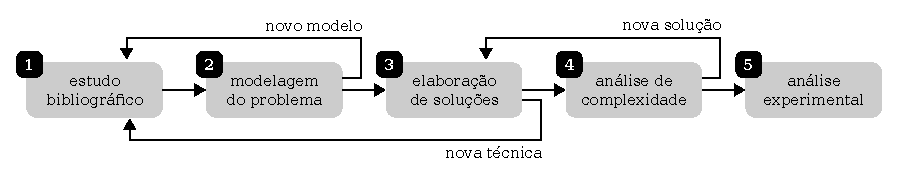
\includegraphics[scale=1]{image/metodologia}
\caption[Ilustração do procedimento metodológico]
    {Ilustração do procedimento metodológico adotado no desenvolvimento deste
    trabalho.
    O processo foi divido em 5 estágios:
    (1) estudo bibliográfico para fundamentar o desenvolvimento de modelos
        representativos do problema;
    (2) modelagem do problema para servir de referência para a elaboração de
        soluções que, se identificadas como inadequadas, podem remeter
        novamente ao estudo bibliográfico;
    (3) elaboração de soluções algorítmicas que serão avaliadas nos próximos
        estágios;
    (4) análise de complexidade das soluções que, quando ineficientes, podem
        remeter a elaboração de uma nova solução e
    (5) análise experimental dos resultados teóricos.}
\label{fig:metodologia}
\end{figure}

A seguir, cada um dos estágios do procedimento metodológico apresentado na
Figura~\ref{fig:metodologia} é descrito.
Na descrição de cada estágio, são considerados, além de seu objetivo, as
possibilidades de evolução de acordo com a ilustração apresentada.

\begin{compactenum}
\item {\bf Estudo bibliográfico}: consiste na busca por bibliografia de
    referência e soluções anteriores para o problema considerado, incluindo
    soluções para problemas similares ou logicamente equivalentes.
    Em relação à evolução temos que:
    \begin{compactenum}[(i)]
    \item o estudo inicial pode levar a um ciclo de busca por soluções que, por
        sua vez, pode remeter ao estudo bibliográfico de outros trabalhos e
    \item dado que a bibliografia levantada é tida como definitiva, o próximo
        estágio a ser considerado é o da criação de um modelo para o problema
        que possa ser utilizado na elaboração de soluções.
    \end{compactenum}
\item {\bf Modelagem do problema}: com base no referencial teórico construído
    no primeiro estágio deve-se criar um modelo matemático que represente o
    problema de forma eficaz.
    Em relação à evolução desse estágio têm-se três opções:
    \begin{compactenum}[(i)]
    \item passar para o estágio de elaboração de soluções quando o modelo é
        eficaz para o problema em questão;
    \item estender a modelagem ao se verificar uma deficiência na abordagem
        encontrada na literatura e
    \item possivelmente, quando a necessidade de extensão ocorre, deve-se
        recorrer novamente ao estudo bibliográfico, pois essas extensões devem
        ser cuidadosamente projetadas e validadas.
    \end{compactenum}
\item {\bf Elaboração de soluções}: a partir do modelo criado no estágio
    anterior, é possível elaborar soluções algorítmicas e aplicar métodos de
    otimização a fim de solucionar o problema redefinido com base no modelo
    matemático construído;
    Em relação à evolução desse estágio têm-se três opções:
    \begin{compactenum}[(i)]
    \item passar para o estágio de análise de complexidade da solução, seja
        essa complexidade associada à necessidade de recursos de tempo ou de
        memória;
    \item estender a solução para subproblemas do modelo a fim de verificar
        propriedades que caracterizam e subsidiam a formação de hipóteses e
    \item possivelmente, quando a necessidade de uma nova técnica ocorre,
        deve-se recorrer novamente ao estudo bibliográfico.
    \end{compactenum}
\item {\bf Análise de complexidade}: cada solução projetada tem um custo de
    implementação associado.
    A princípio, este custo não deve inviabilizar a utilização da solução em
    termos de tempo e memória, dentre outros recursos, necessários para
    resolver o problema em questão.
    Em relação à evolução temos que:
    \begin{compactenum}[(i)]
    \item se as complexidades envolvidas satisfizerem os requisitos, então
        evolui-se para o estágio de implementação das soluções de forma
        integrada e
    \item se a complexidade for proibitiva, é necessário voltar ao estágio de
        elaboração para construção de uma outra solução.
    \end{compactenum}
\item {\bf Análise experimental}: se o estágio de análise de complexidade
    fomenta a utilização da solução proposta, deve-se realizar experimentos com
    dados reais para validar a solução, ou aplicá-las à instâncias do modelo a
    fim de extrair conjecturas acerca das propriedades do modelo que indiquem a
    validade da solução.
\end{compactenum}

%%%%%%%%%%%%%%%%%%%%%%%%%%%%%%%%%%%%%%%%%%%%%%%%%%%%%%%%%%%%%%%%%%%%%%%%%%%%%%%
%% FIM CAPÍTULO                                                              %%
%%%%%%%%%%%%%%%%%%%%%%%%%%%%%%%%%%%%%%%%%%%%%%%%%%%%%%%%%%%%%%%%%%%%%%%%%%%%%%%
 % Introdução (apresentação do trabalho)
%%%%%%%%%%%%%%%%%%%%%%%%%%%%%%%%%%%%%%%%%%%%%%%%%%%%%%%%%%%%%%%%%%%%%%%%%%%%%%%
%% INÍCIO CAPÍTULO                                                           %%
%%%%%%%%%%%%%%%%%%%%%%%%%%%%%%%%%%%%%%%%%%%%%%%%%%%%%%%%%%%%%%%%%%%%%%%%%%%%%%%

\chapter{Levantamento bibliográfico}
\label{cap:2:fundamentacao}

\citacao{%
We can only see a short distance ahead,\\
but we can see plenty there that needs to be done.}
{Alan Mathison Turing}

O entendimento dos fundamentos...

Este Capítulo está organizado da seguinte forma...

% =========================================================================== %
\section{Introdução}
\label{sec:2:introducao}

\citep{brassard1996fundamentals}

% =========================================================================== %
\section{Fundamentação}
\label{sec:2:fundamentacao}

\begin{definicao}[Grafo direcionado com pesos]\label{def:grafo}
\index{grafo!definicao@definição}%
\index{grafo!direcionado com pesos}%
\citep{cormen2009algorithms}
Um grafo direcionado com pesos $G$ é composto por uma tripla ordenada
$G=\langle N, E, \omega \rangle$, onde $N$ representa o conjunto de vértices
(ou nós) do grafo e $E$ o conjunto de arestas ao qual se atribui as seguintes
propriedades:
\begin{inparaenum}[(i)]
\item cada aresta é composta por um par ordenado de nós $(v_1,v_2)$, que indica
    que existe uma ligação saindo do nó $v_1$ em direção ao nó $v_2$ e
\item para cada aresta $e \in E$ existe um peso que é associado por uma função
    $\omega(\cdot)$, que realiza o mapeamento dos pesos de cada aresta para um
    número real, ou seja, $\omega \colon E\mapsto\mathbb{R}$.
\end{inparaenum}
\end{definicao}

\begin{algoritmo}[Cálculo dos graus de entrada e saída de cada nó]
\label{alg:graus}
\index{algoritmo!graus()}%
É possível calcular os graus de entrada e saída de cada nó da rede
de forma iterativa com base na representação por lista de adjacência.

\begin{algorithmic}[1]
\REQUIRE{graus$(L)$}
\STATE\COMMENT{Lista de adjacência $L$ de um grafo direcionado $G=\langle
    N,E\rangle$.}
\STATE $g_\text{in} \leftarrow \text{novo-vetor}(|N|, 0)$
    \COMMENT{Vetor de $|N|$ posições preenchidas com zero.}
\STATE $g_\text{out} \leftarrow \text{novo-vetor}(|N|, 0)$
\FOR{$i$ de $1$ até $|N|$}
    \FORALL{$(v_j,p) \in L[i]$}
        \STATE\COMMENT{Nó adjacente $v_j$ e peso $p$ da aresta.}
        \STATE $g_\text{out}[i] \leftarrow g_\text{out}[i] + 1$
        \STATE $g_\text{in}[j] \leftarrow g_\text{in}[j] + 1$
    \ENDFOR
\ENDFOR
\RETURN $\langle g_\text{in}, g_\text{out} \rangle$
\COMMENT{Vetores com os graus de entrada e saída de cada nó da rede.}
\end{algorithmic}
Considera-se que os vetores $g_\text{in}$ e $g_\text{out}$ são indexados a
partir de 1.
A complexidade do algoritmo é da ordem de 
$\Theta(n\operatorname{E}\{\mathcal{G}^\text{out}\})$ em tempo e $\Theta(n)$ em
memória.
\end{algoritmo}

% =========================================================================== %
\section{Objetivos específicos}
\label{sec:2:objetivos}


% =========================================================================== %
\section{Metodologia}
\label{sec:2:metodologia}

O procedimento metodológico utilizado no desenvolvimento deste trabalho possui
uma abordagem dividida em 5 estágios.
Esses estágios são ordenados em uma sequência em que é permitida uma evolução
com ciclos, cuja relação é descrita na Figura~\ref{fig:metodologia}.

\begin{figure}[ht]
\index{metodologia!procedimento}
\centering
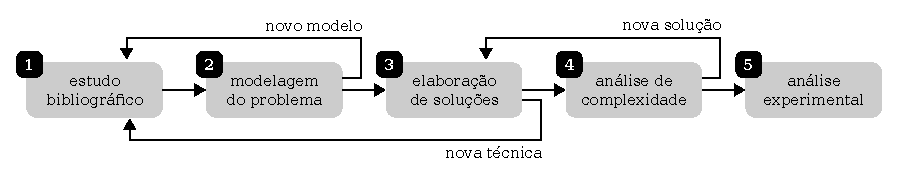
\includegraphics[scale=1]{image/metodologia}
\caption[Ilustração do procedimento metodológico]
    {Ilustração do procedimento metodológico adotado no desenvolvimento deste
    trabalho.
    O processo foi divido em 5 estágios:
    (1) estudo bibliográfico para fundamentar o desenvolvimento de modelos
        representativos do problema;
    (2) modelagem do problema para servir de referência para a elaboração de
        soluções que, se identificadas como inadequadas, podem remeter
        novamente ao estudo bibliográfico;
    (3) elaboração de soluções algorítmicas que serão avaliadas nos próximos
        estágios;
    (4) análise de complexidade das soluções que, quando ineficientes, podem
        remeter a elaboração de uma nova solução e
    (5) análise experimental dos resultados teóricos.}
\label{fig:metodologia}
\end{figure}

A seguir, cada um dos estágios do procedimento metodológico apresentado na
Figura~\ref{fig:metodologia} é descrito.
Na descrição de cada estágio, são considerados, além de seu objetivo, as
possibilidades de evolução de acordo com a ilustração apresentada.

\begin{compactenum}
\item {\bf Estudo bibliográfico}: consiste na busca por bibliografia de
    referência e soluções anteriores para o problema considerado, incluindo
    soluções para problemas similares ou logicamente equivalentes.
    Em relação à evolução temos que:
    \begin{compactenum}[(i)]
    \item o estudo inicial pode levar a um ciclo de busca por soluções que, por
        sua vez, pode remeter ao estudo bibliográfico de outros trabalhos e
    \item dado que a bibliografia levantada é tida como definitiva, o próximo
        estágio a ser considerado é o da criação de um modelo para o problema
        que possa ser utilizado na elaboração de soluções.
    \end{compactenum}
\item {\bf Modelagem do problema}: com base no referencial teórico construído
    no primeiro estágio deve-se criar um modelo matemático que represente o
    problema de forma eficaz.
    Em relação à evolução desse estágio têm-se três opções:
    \begin{compactenum}[(i)]
    \item passar para o estágio de elaboração de soluções quando o modelo é
        eficaz para o problema em questão;
    \item estender a modelagem ao se verificar uma deficiência na abordagem
        encontrada na literatura e
    \item possivelmente, quando a necessidade de extensão ocorre, deve-se
        recorrer novamente ao estudo bibliográfico, pois essas extensões devem
        ser cuidadosamente projetadas e validadas.
    \end{compactenum}
\item {\bf Elaboração de soluções}: a partir do modelo criado no estágio
    anterior, é possível elaborar soluções algorítmicas e aplicar métodos de
    otimização a fim de solucionar o problema redefinido com base no modelo
    matemático construído;
    Em relação à evolução desse estágio têm-se três opções:
    \begin{compactenum}[(i)]
    \item passar para o estágio de análise de complexidade da solução, seja
        essa complexidade associada à necessidade de recursos de tempo ou de
        memória;
    \item estender a solução para subproblemas do modelo a fim de verificar
        propriedades que caracterizam e subsidiam a formação de hipóteses e
    \item possivelmente, quando a necessidade de uma nova técnica ocorre,
        deve-se recorrer novamente ao estudo bibliográfico.
    \end{compactenum}
\item {\bf Análise de complexidade}: cada solução projetada tem um custo de
    implementação associado.
    A princípio, este custo não deve inviabilizar a utilização da solução em
    termos de tempo e memória, dentre outros recursos, necessários para
    resolver o problema em questão.
    Em relação à evolução temos que:
    \begin{compactenum}[(i)]
    \item se as complexidades envolvidas satisfizerem os requisitos, então
        evolui-se para o estágio de implementação das soluções de forma
        integrada e
    \item se a complexidade for proibitiva, é necessário voltar ao estágio de
        elaboração para construção de uma outra solução.
    \end{compactenum}
\item {\bf Análise experimental}: se o estágio de análise de complexidade
    fomenta a utilização da solução proposta, deve-se realizar experimentos com
    dados reais para validar a solução, ou aplicá-las à instâncias do modelo a
    fim de extrair conjecturas acerca das propriedades do modelo que indiquem a
    validade da solução.
\end{compactenum}

%%%%%%%%%%%%%%%%%%%%%%%%%%%%%%%%%%%%%%%%%%%%%%%%%%%%%%%%%%%%%%%%%%%%%%%%%%%%%%%
%% FIM CAPÍTULO                                                              %%
%%%%%%%%%%%%%%%%%%%%%%%%%%%%%%%%%%%%%%%%%%%%%%%%%%%%%%%%%%%%%%%%%%%%%%%%%%%%%%%
 % Levantamento bibliográfico e metodologia
%%%%%%%%%%%%%%%%%%%%%%%%%%%%%%%%%%%%%%%%%%%%%%%%%%%%%%%%%%%%%%%%%%%%%%%%%%%%%%%
%% INÍCIO CAPÍTULO                                                           %%
%%%%%%%%%%%%%%%%%%%%%%%%%%%%%%%%%%%%%%%%%%%%%%%%%%%%%%%%%%%%%%%%%%%%%%%%%%%%%%%

\chapter{Levantamento bibliográfico}
\label{cap:2:fundamentacao}

\citacao{%
We can only see a short distance ahead,\\
but we can see plenty there that needs to be done.}
{Alan Mathison Turing}

O entendimento dos fundamentos...

Este Capítulo está organizado da seguinte forma...

% =========================================================================== %
\section{Introdução}
\label{sec:2:introducao}

\citep{brassard1996fundamentals}

% =========================================================================== %
\section{Fundamentação}
\label{sec:2:fundamentacao}

\begin{definicao}[Grafo direcionado com pesos]\label{def:grafo}
\index{grafo!definicao@definição}%
\index{grafo!direcionado com pesos}%
\citep{cormen2009algorithms}
Um grafo direcionado com pesos $G$ é composto por uma tripla ordenada
$G=\langle N, E, \omega \rangle$, onde $N$ representa o conjunto de vértices
(ou nós) do grafo e $E$ o conjunto de arestas ao qual se atribui as seguintes
propriedades:
\begin{inparaenum}[(i)]
\item cada aresta é composta por um par ordenado de nós $(v_1,v_2)$, que indica
    que existe uma ligação saindo do nó $v_1$ em direção ao nó $v_2$ e
\item para cada aresta $e \in E$ existe um peso que é associado por uma função
    $\omega(\cdot)$, que realiza o mapeamento dos pesos de cada aresta para um
    número real, ou seja, $\omega \colon E\mapsto\mathbb{R}$.
\end{inparaenum}
\end{definicao}

\begin{algoritmo}[Cálculo dos graus de entrada e saída de cada nó]
\label{alg:graus}
\index{algoritmo!graus()}%
É possível calcular os graus de entrada e saída de cada nó da rede
de forma iterativa com base na representação por lista de adjacência.

\begin{algorithmic}[1]
\REQUIRE{graus$(L)$}
\STATE\COMMENT{Lista de adjacência $L$ de um grafo direcionado $G=\langle
    N,E\rangle$.}
\STATE $g_\text{in} \leftarrow \text{novo-vetor}(|N|, 0)$
    \COMMENT{Vetor de $|N|$ posições preenchidas com zero.}
\STATE $g_\text{out} \leftarrow \text{novo-vetor}(|N|, 0)$
\FOR{$i$ de $1$ até $|N|$}
    \FORALL{$(v_j,p) \in L[i]$}
        \STATE\COMMENT{Nó adjacente $v_j$ e peso $p$ da aresta.}
        \STATE $g_\text{out}[i] \leftarrow g_\text{out}[i] + 1$
        \STATE $g_\text{in}[j] \leftarrow g_\text{in}[j] + 1$
    \ENDFOR
\ENDFOR
\RETURN $\langle g_\text{in}, g_\text{out} \rangle$
\COMMENT{Vetores com os graus de entrada e saída de cada nó da rede.}
\end{algorithmic}
Considera-se que os vetores $g_\text{in}$ e $g_\text{out}$ são indexados a
partir de 1.
A complexidade do algoritmo é da ordem de 
$\Theta(n\operatorname{E}\{\mathcal{G}^\text{out}\})$ em tempo e $\Theta(n)$ em
memória.
\end{algoritmo}

% =========================================================================== %
\section{Objetivos específicos}
\label{sec:2:objetivos}


% =========================================================================== %
\section{Metodologia}
\label{sec:2:metodologia}

O procedimento metodológico utilizado no desenvolvimento deste trabalho possui
uma abordagem dividida em 5 estágios.
Esses estágios são ordenados em uma sequência em que é permitida uma evolução
com ciclos, cuja relação é descrita na Figura~\ref{fig:metodologia}.

\begin{figure}[ht]
\index{metodologia!procedimento}
\centering
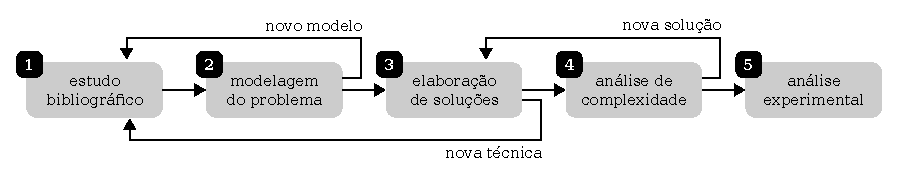
\includegraphics[scale=1]{image/metodologia}
\caption[Ilustração do procedimento metodológico]
    {Ilustração do procedimento metodológico adotado no desenvolvimento deste
    trabalho.
    O processo foi divido em 5 estágios:
    (1) estudo bibliográfico para fundamentar o desenvolvimento de modelos
        representativos do problema;
    (2) modelagem do problema para servir de referência para a elaboração de
        soluções que, se identificadas como inadequadas, podem remeter
        novamente ao estudo bibliográfico;
    (3) elaboração de soluções algorítmicas que serão avaliadas nos próximos
        estágios;
    (4) análise de complexidade das soluções que, quando ineficientes, podem
        remeter a elaboração de uma nova solução e
    (5) análise experimental dos resultados teóricos.}
\label{fig:metodologia}
\end{figure}

A seguir, cada um dos estágios do procedimento metodológico apresentado na
Figura~\ref{fig:metodologia} é descrito.
Na descrição de cada estágio, são considerados, além de seu objetivo, as
possibilidades de evolução de acordo com a ilustração apresentada.

\begin{compactenum}
\item {\bf Estudo bibliográfico}: consiste na busca por bibliografia de
    referência e soluções anteriores para o problema considerado, incluindo
    soluções para problemas similares ou logicamente equivalentes.
    Em relação à evolução temos que:
    \begin{compactenum}[(i)]
    \item o estudo inicial pode levar a um ciclo de busca por soluções que, por
        sua vez, pode remeter ao estudo bibliográfico de outros trabalhos e
    \item dado que a bibliografia levantada é tida como definitiva, o próximo
        estágio a ser considerado é o da criação de um modelo para o problema
        que possa ser utilizado na elaboração de soluções.
    \end{compactenum}
\item {\bf Modelagem do problema}: com base no referencial teórico construído
    no primeiro estágio deve-se criar um modelo matemático que represente o
    problema de forma eficaz.
    Em relação à evolução desse estágio têm-se três opções:
    \begin{compactenum}[(i)]
    \item passar para o estágio de elaboração de soluções quando o modelo é
        eficaz para o problema em questão;
    \item estender a modelagem ao se verificar uma deficiência na abordagem
        encontrada na literatura e
    \item possivelmente, quando a necessidade de extensão ocorre, deve-se
        recorrer novamente ao estudo bibliográfico, pois essas extensões devem
        ser cuidadosamente projetadas e validadas.
    \end{compactenum}
\item {\bf Elaboração de soluções}: a partir do modelo criado no estágio
    anterior, é possível elaborar soluções algorítmicas e aplicar métodos de
    otimização a fim de solucionar o problema redefinido com base no modelo
    matemático construído;
    Em relação à evolução desse estágio têm-se três opções:
    \begin{compactenum}[(i)]
    \item passar para o estágio de análise de complexidade da solução, seja
        essa complexidade associada à necessidade de recursos de tempo ou de
        memória;
    \item estender a solução para subproblemas do modelo a fim de verificar
        propriedades que caracterizam e subsidiam a formação de hipóteses e
    \item possivelmente, quando a necessidade de uma nova técnica ocorre,
        deve-se recorrer novamente ao estudo bibliográfico.
    \end{compactenum}
\item {\bf Análise de complexidade}: cada solução projetada tem um custo de
    implementação associado.
    A princípio, este custo não deve inviabilizar a utilização da solução em
    termos de tempo e memória, dentre outros recursos, necessários para
    resolver o problema em questão.
    Em relação à evolução temos que:
    \begin{compactenum}[(i)]
    \item se as complexidades envolvidas satisfizerem os requisitos, então
        evolui-se para o estágio de implementação das soluções de forma
        integrada e
    \item se a complexidade for proibitiva, é necessário voltar ao estágio de
        elaboração para construção de uma outra solução.
    \end{compactenum}
\item {\bf Análise experimental}: se o estágio de análise de complexidade
    fomenta a utilização da solução proposta, deve-se realizar experimentos com
    dados reais para validar a solução, ou aplicá-las à instâncias do modelo a
    fim de extrair conjecturas acerca das propriedades do modelo que indiquem a
    validade da solução.
\end{compactenum}

%%%%%%%%%%%%%%%%%%%%%%%%%%%%%%%%%%%%%%%%%%%%%%%%%%%%%%%%%%%%%%%%%%%%%%%%%%%%%%%
%% FIM CAPÍTULO                                                              %%
%%%%%%%%%%%%%%%%%%%%%%%%%%%%%%%%%%%%%%%%%%%%%%%%%%%%%%%%%%%%%%%%%%%%%%%%%%%%%%%
 % Desenvolvimento e resultados do trabalho
%%%%%%%%%%%%%%%%%%%%%%%%%%%%%%%%%%%%%%%%%%%%%%%%%%%%%%%%%%%%%%%%%%%%%%%%%%%%%%%
%% INÍCIO CAPÍTULO                                                           %%
%%%%%%%%%%%%%%%%%%%%%%%%%%%%%%%%%%%%%%%%%%%%%%%%%%%%%%%%%%%%%%%%%%%%%%%%%%%%%%%

\chapter{Levantamento bibliográfico}
\label{cap:2:fundamentacao}

\citacao{%
We can only see a short distance ahead,\\
but we can see plenty there that needs to be done.}
{Alan Mathison Turing}

O entendimento dos fundamentos...

Este Capítulo está organizado da seguinte forma...

% =========================================================================== %
\section{Introdução}
\label{sec:2:introducao}

\citep{brassard1996fundamentals}

% =========================================================================== %
\section{Fundamentação}
\label{sec:2:fundamentacao}

\begin{definicao}[Grafo direcionado com pesos]\label{def:grafo}
\index{grafo!definicao@definição}%
\index{grafo!direcionado com pesos}%
\citep{cormen2009algorithms}
Um grafo direcionado com pesos $G$ é composto por uma tripla ordenada
$G=\langle N, E, \omega \rangle$, onde $N$ representa o conjunto de vértices
(ou nós) do grafo e $E$ o conjunto de arestas ao qual se atribui as seguintes
propriedades:
\begin{inparaenum}[(i)]
\item cada aresta é composta por um par ordenado de nós $(v_1,v_2)$, que indica
    que existe uma ligação saindo do nó $v_1$ em direção ao nó $v_2$ e
\item para cada aresta $e \in E$ existe um peso que é associado por uma função
    $\omega(\cdot)$, que realiza o mapeamento dos pesos de cada aresta para um
    número real, ou seja, $\omega \colon E\mapsto\mathbb{R}$.
\end{inparaenum}
\end{definicao}

\begin{algoritmo}[Cálculo dos graus de entrada e saída de cada nó]
\label{alg:graus}
\index{algoritmo!graus()}%
É possível calcular os graus de entrada e saída de cada nó da rede
de forma iterativa com base na representação por lista de adjacência.

\begin{algorithmic}[1]
\REQUIRE{graus$(L)$}
\STATE\COMMENT{Lista de adjacência $L$ de um grafo direcionado $G=\langle
    N,E\rangle$.}
\STATE $g_\text{in} \leftarrow \text{novo-vetor}(|N|, 0)$
    \COMMENT{Vetor de $|N|$ posições preenchidas com zero.}
\STATE $g_\text{out} \leftarrow \text{novo-vetor}(|N|, 0)$
\FOR{$i$ de $1$ até $|N|$}
    \FORALL{$(v_j,p) \in L[i]$}
        \STATE\COMMENT{Nó adjacente $v_j$ e peso $p$ da aresta.}
        \STATE $g_\text{out}[i] \leftarrow g_\text{out}[i] + 1$
        \STATE $g_\text{in}[j] \leftarrow g_\text{in}[j] + 1$
    \ENDFOR
\ENDFOR
\RETURN $\langle g_\text{in}, g_\text{out} \rangle$
\COMMENT{Vetores com os graus de entrada e saída de cada nó da rede.}
\end{algorithmic}
Considera-se que os vetores $g_\text{in}$ e $g_\text{out}$ são indexados a
partir de 1.
A complexidade do algoritmo é da ordem de 
$\Theta(n\operatorname{E}\{\mathcal{G}^\text{out}\})$ em tempo e $\Theta(n)$ em
memória.
\end{algoritmo}

% =========================================================================== %
\section{Objetivos específicos}
\label{sec:2:objetivos}


% =========================================================================== %
\section{Metodologia}
\label{sec:2:metodologia}

O procedimento metodológico utilizado no desenvolvimento deste trabalho possui
uma abordagem dividida em 5 estágios.
Esses estágios são ordenados em uma sequência em que é permitida uma evolução
com ciclos, cuja relação é descrita na Figura~\ref{fig:metodologia}.

\begin{figure}[ht]
\index{metodologia!procedimento}
\centering
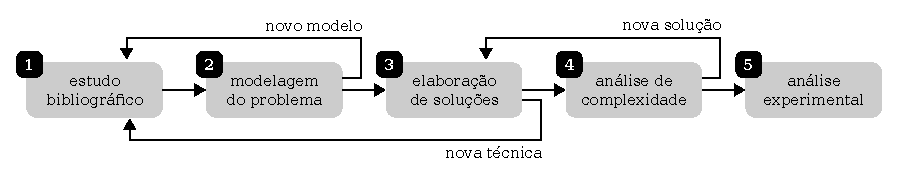
\includegraphics[scale=1]{image/metodologia}
\caption[Ilustração do procedimento metodológico]
    {Ilustração do procedimento metodológico adotado no desenvolvimento deste
    trabalho.
    O processo foi divido em 5 estágios:
    (1) estudo bibliográfico para fundamentar o desenvolvimento de modelos
        representativos do problema;
    (2) modelagem do problema para servir de referência para a elaboração de
        soluções que, se identificadas como inadequadas, podem remeter
        novamente ao estudo bibliográfico;
    (3) elaboração de soluções algorítmicas que serão avaliadas nos próximos
        estágios;
    (4) análise de complexidade das soluções que, quando ineficientes, podem
        remeter a elaboração de uma nova solução e
    (5) análise experimental dos resultados teóricos.}
\label{fig:metodologia}
\end{figure}

A seguir, cada um dos estágios do procedimento metodológico apresentado na
Figura~\ref{fig:metodologia} é descrito.
Na descrição de cada estágio, são considerados, além de seu objetivo, as
possibilidades de evolução de acordo com a ilustração apresentada.

\begin{compactenum}
\item {\bf Estudo bibliográfico}: consiste na busca por bibliografia de
    referência e soluções anteriores para o problema considerado, incluindo
    soluções para problemas similares ou logicamente equivalentes.
    Em relação à evolução temos que:
    \begin{compactenum}[(i)]
    \item o estudo inicial pode levar a um ciclo de busca por soluções que, por
        sua vez, pode remeter ao estudo bibliográfico de outros trabalhos e
    \item dado que a bibliografia levantada é tida como definitiva, o próximo
        estágio a ser considerado é o da criação de um modelo para o problema
        que possa ser utilizado na elaboração de soluções.
    \end{compactenum}
\item {\bf Modelagem do problema}: com base no referencial teórico construído
    no primeiro estágio deve-se criar um modelo matemático que represente o
    problema de forma eficaz.
    Em relação à evolução desse estágio têm-se três opções:
    \begin{compactenum}[(i)]
    \item passar para o estágio de elaboração de soluções quando o modelo é
        eficaz para o problema em questão;
    \item estender a modelagem ao se verificar uma deficiência na abordagem
        encontrada na literatura e
    \item possivelmente, quando a necessidade de extensão ocorre, deve-se
        recorrer novamente ao estudo bibliográfico, pois essas extensões devem
        ser cuidadosamente projetadas e validadas.
    \end{compactenum}
\item {\bf Elaboração de soluções}: a partir do modelo criado no estágio
    anterior, é possível elaborar soluções algorítmicas e aplicar métodos de
    otimização a fim de solucionar o problema redefinido com base no modelo
    matemático construído;
    Em relação à evolução desse estágio têm-se três opções:
    \begin{compactenum}[(i)]
    \item passar para o estágio de análise de complexidade da solução, seja
        essa complexidade associada à necessidade de recursos de tempo ou de
        memória;
    \item estender a solução para subproblemas do modelo a fim de verificar
        propriedades que caracterizam e subsidiam a formação de hipóteses e
    \item possivelmente, quando a necessidade de uma nova técnica ocorre,
        deve-se recorrer novamente ao estudo bibliográfico.
    \end{compactenum}
\item {\bf Análise de complexidade}: cada solução projetada tem um custo de
    implementação associado.
    A princípio, este custo não deve inviabilizar a utilização da solução em
    termos de tempo e memória, dentre outros recursos, necessários para
    resolver o problema em questão.
    Em relação à evolução temos que:
    \begin{compactenum}[(i)]
    \item se as complexidades envolvidas satisfizerem os requisitos, então
        evolui-se para o estágio de implementação das soluções de forma
        integrada e
    \item se a complexidade for proibitiva, é necessário voltar ao estágio de
        elaboração para construção de uma outra solução.
    \end{compactenum}
\item {\bf Análise experimental}: se o estágio de análise de complexidade
    fomenta a utilização da solução proposta, deve-se realizar experimentos com
    dados reais para validar a solução, ou aplicá-las à instâncias do modelo a
    fim de extrair conjecturas acerca das propriedades do modelo que indiquem a
    validade da solução.
\end{compactenum}

%%%%%%%%%%%%%%%%%%%%%%%%%%%%%%%%%%%%%%%%%%%%%%%%%%%%%%%%%%%%%%%%%%%%%%%%%%%%%%%
%% FIM CAPÍTULO                                                              %%
%%%%%%%%%%%%%%%%%%%%%%%%%%%%%%%%%%%%%%%%%%%%%%%%%%%%%%%%%%%%%%%%%%%%%%%%%%%%%%%
 % Conclusões e trabalhos futuros

%%%%%%%%%%%%%%%%%%%%%%%%%%%%%%%%%%%%%%%%%%%%%%%%%%%%%%%%%%%%%%%%%%%%%%%%%%%%%
%% APÊNDICE, BILIOGRAFIA E ÍNDICE REMISSIVO                                %%
%%%%%%%%%%%%%%%%%%%%%%%%%%%%%%%%%%%%%%%%%%%%%%%%%%%%%%%%%%%%%%%%%%%%%%%%%%%%%
\appendix
%%%%%%%%%%%%%%%%%%%%%%%%%%%%%%%%%%%%%%%%%%%%%%%%%%%%%%%%%%%%%%%%%%%%%%%%%%%%%%%
%% INÍCIO CAPÍTULO                                                           %%
%%%%%%%%%%%%%%%%%%%%%%%%%%%%%%%%%%%%%%%%%%%%%%%%%%%%%%%%%%%%%%%%%%%%%%%%%%%%%%%

\chapter{Levantamento bibliográfico}
\label{cap:2:fundamentacao}

\citacao{%
We can only see a short distance ahead,\\
but we can see plenty there that needs to be done.}
{Alan Mathison Turing}

O entendimento dos fundamentos...

Este Capítulo está organizado da seguinte forma...

% =========================================================================== %
\section{Introdução}
\label{sec:2:introducao}

\citep{brassard1996fundamentals}

% =========================================================================== %
\section{Fundamentação}
\label{sec:2:fundamentacao}

\begin{definicao}[Grafo direcionado com pesos]\label{def:grafo}
\index{grafo!definicao@definição}%
\index{grafo!direcionado com pesos}%
\citep{cormen2009algorithms}
Um grafo direcionado com pesos $G$ é composto por uma tripla ordenada
$G=\langle N, E, \omega \rangle$, onde $N$ representa o conjunto de vértices
(ou nós) do grafo e $E$ o conjunto de arestas ao qual se atribui as seguintes
propriedades:
\begin{inparaenum}[(i)]
\item cada aresta é composta por um par ordenado de nós $(v_1,v_2)$, que indica
    que existe uma ligação saindo do nó $v_1$ em direção ao nó $v_2$ e
\item para cada aresta $e \in E$ existe um peso que é associado por uma função
    $\omega(\cdot)$, que realiza o mapeamento dos pesos de cada aresta para um
    número real, ou seja, $\omega \colon E\mapsto\mathbb{R}$.
\end{inparaenum}
\end{definicao}

\begin{algoritmo}[Cálculo dos graus de entrada e saída de cada nó]
\label{alg:graus}
\index{algoritmo!graus()}%
É possível calcular os graus de entrada e saída de cada nó da rede
de forma iterativa com base na representação por lista de adjacência.

\begin{algorithmic}[1]
\REQUIRE{graus$(L)$}
\STATE\COMMENT{Lista de adjacência $L$ de um grafo direcionado $G=\langle
    N,E\rangle$.}
\STATE $g_\text{in} \leftarrow \text{novo-vetor}(|N|, 0)$
    \COMMENT{Vetor de $|N|$ posições preenchidas com zero.}
\STATE $g_\text{out} \leftarrow \text{novo-vetor}(|N|, 0)$
\FOR{$i$ de $1$ até $|N|$}
    \FORALL{$(v_j,p) \in L[i]$}
        \STATE\COMMENT{Nó adjacente $v_j$ e peso $p$ da aresta.}
        \STATE $g_\text{out}[i] \leftarrow g_\text{out}[i] + 1$
        \STATE $g_\text{in}[j] \leftarrow g_\text{in}[j] + 1$
    \ENDFOR
\ENDFOR
\RETURN $\langle g_\text{in}, g_\text{out} \rangle$
\COMMENT{Vetores com os graus de entrada e saída de cada nó da rede.}
\end{algorithmic}
Considera-se que os vetores $g_\text{in}$ e $g_\text{out}$ são indexados a
partir de 1.
A complexidade do algoritmo é da ordem de 
$\Theta(n\operatorname{E}\{\mathcal{G}^\text{out}\})$ em tempo e $\Theta(n)$ em
memória.
\end{algoritmo}

% =========================================================================== %
\section{Objetivos específicos}
\label{sec:2:objetivos}


% =========================================================================== %
\section{Metodologia}
\label{sec:2:metodologia}

O procedimento metodológico utilizado no desenvolvimento deste trabalho possui
uma abordagem dividida em 5 estágios.
Esses estágios são ordenados em uma sequência em que é permitida uma evolução
com ciclos, cuja relação é descrita na Figura~\ref{fig:metodologia}.

\begin{figure}[ht]
\index{metodologia!procedimento}
\centering
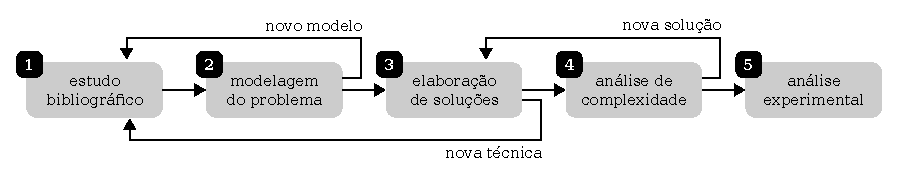
\includegraphics[scale=1]{image/metodologia}
\caption[Ilustração do procedimento metodológico]
    {Ilustração do procedimento metodológico adotado no desenvolvimento deste
    trabalho.
    O processo foi divido em 5 estágios:
    (1) estudo bibliográfico para fundamentar o desenvolvimento de modelos
        representativos do problema;
    (2) modelagem do problema para servir de referência para a elaboração de
        soluções que, se identificadas como inadequadas, podem remeter
        novamente ao estudo bibliográfico;
    (3) elaboração de soluções algorítmicas que serão avaliadas nos próximos
        estágios;
    (4) análise de complexidade das soluções que, quando ineficientes, podem
        remeter a elaboração de uma nova solução e
    (5) análise experimental dos resultados teóricos.}
\label{fig:metodologia}
\end{figure}

A seguir, cada um dos estágios do procedimento metodológico apresentado na
Figura~\ref{fig:metodologia} é descrito.
Na descrição de cada estágio, são considerados, além de seu objetivo, as
possibilidades de evolução de acordo com a ilustração apresentada.

\begin{compactenum}
\item {\bf Estudo bibliográfico}: consiste na busca por bibliografia de
    referência e soluções anteriores para o problema considerado, incluindo
    soluções para problemas similares ou logicamente equivalentes.
    Em relação à evolução temos que:
    \begin{compactenum}[(i)]
    \item o estudo inicial pode levar a um ciclo de busca por soluções que, por
        sua vez, pode remeter ao estudo bibliográfico de outros trabalhos e
    \item dado que a bibliografia levantada é tida como definitiva, o próximo
        estágio a ser considerado é o da criação de um modelo para o problema
        que possa ser utilizado na elaboração de soluções.
    \end{compactenum}
\item {\bf Modelagem do problema}: com base no referencial teórico construído
    no primeiro estágio deve-se criar um modelo matemático que represente o
    problema de forma eficaz.
    Em relação à evolução desse estágio têm-se três opções:
    \begin{compactenum}[(i)]
    \item passar para o estágio de elaboração de soluções quando o modelo é
        eficaz para o problema em questão;
    \item estender a modelagem ao se verificar uma deficiência na abordagem
        encontrada na literatura e
    \item possivelmente, quando a necessidade de extensão ocorre, deve-se
        recorrer novamente ao estudo bibliográfico, pois essas extensões devem
        ser cuidadosamente projetadas e validadas.
    \end{compactenum}
\item {\bf Elaboração de soluções}: a partir do modelo criado no estágio
    anterior, é possível elaborar soluções algorítmicas e aplicar métodos de
    otimização a fim de solucionar o problema redefinido com base no modelo
    matemático construído;
    Em relação à evolução desse estágio têm-se três opções:
    \begin{compactenum}[(i)]
    \item passar para o estágio de análise de complexidade da solução, seja
        essa complexidade associada à necessidade de recursos de tempo ou de
        memória;
    \item estender a solução para subproblemas do modelo a fim de verificar
        propriedades que caracterizam e subsidiam a formação de hipóteses e
    \item possivelmente, quando a necessidade de uma nova técnica ocorre,
        deve-se recorrer novamente ao estudo bibliográfico.
    \end{compactenum}
\item {\bf Análise de complexidade}: cada solução projetada tem um custo de
    implementação associado.
    A princípio, este custo não deve inviabilizar a utilização da solução em
    termos de tempo e memória, dentre outros recursos, necessários para
    resolver o problema em questão.
    Em relação à evolução temos que:
    \begin{compactenum}[(i)]
    \item se as complexidades envolvidas satisfizerem os requisitos, então
        evolui-se para o estágio de implementação das soluções de forma
        integrada e
    \item se a complexidade for proibitiva, é necessário voltar ao estágio de
        elaboração para construção de uma outra solução.
    \end{compactenum}
\item {\bf Análise experimental}: se o estágio de análise de complexidade
    fomenta a utilização da solução proposta, deve-se realizar experimentos com
    dados reais para validar a solução, ou aplicá-las à instâncias do modelo a
    fim de extrair conjecturas acerca das propriedades do modelo que indiquem a
    validade da solução.
\end{compactenum}

%%%%%%%%%%%%%%%%%%%%%%%%%%%%%%%%%%%%%%%%%%%%%%%%%%%%%%%%%%%%%%%%%%%%%%%%%%%%%%%
%% FIM CAPÍTULO                                                              %%
%%%%%%%%%%%%%%%%%%%%%%%%%%%%%%%%%%%%%%%%%%%%%%%%%%%%%%%%%%%%%%%%%%%%%%%%%%%%%%%


\if\doctype\doctypem           % Se é do tipo monografia
\backmatter
\fi

\limparpagina
%\nocite{*}
\bibliographystyle{labepi}
\bibliography{content/bibliography}
\addcontentsline{toc}{chapter}{\bibname}

\limparpagina
\markboth{Índice Remissivo}{Índice Remissivo}
\printindex

\end{document}

%%%%%%%%%%%%%%%%%%%%%%%%%%%%%%%%%%%%%%%%%%%%%%%%%%%%%%%%%%%%%%%%%%%%%%%%%%%%%
%% FIM DO DOCUMENTO                                                        %%
%%%%%%%%%%%%%%%%%%%%%%%%%%%%%%%%%%%%%%%%%%%%%%%%%%%%%%%%%%%%%%%%%%%%%%%%%%%%%
